\chapter*{Spin-phonon coupling}

\section*{Transport}
I want to allow for the propagation of excitations through the chain. The first step towards this is constructing a Hamiltonian which describes the dynamics of a system of Rydberg atoms, where one atom is excited, hence restricting ourselves to the single excitation subspace. The general coupling between the atoms arises from the interaction between the dipole moments of the atoms,
\begin{align*}
    V&=\sum_\mathbf{r}V(\mathbf{r})\\
    \text{with}\quad V(\mathbf{r})&= V_0\,\left(\frac{\mathbf{\hat{d}}_1\cdot\mathbf{\hat{d}}_2}{r^3}-3\,\frac{(\mathbf{r}\cdot \mathbf{\hat{d}}_1)(\mathbf{r}\cdot \mathbf{\hat{d}}_2)}{r^5}\right).
\end{align*}
Each individual atom is characterized by its position in the lattice and its atomic energy level which is captured by the non-interacting Hamiltonian $H_0$. The total Hamiltonian thus reads
\begin{align*}
    H = H_0 + V
\end{align*}
We will investigate the system in a regime, where the coupling due to the dipole forces is much smaller than the energy gap $\Delta$, which separates the energy of the atoms from their next higher and lower states, i.e. $\lVert V \rVert\ll\Delta$. In order to gain an approximate effective Hamiltonian, which acts in a closed way on the one excitation subspace, I will perform a Schrieffer-Wolff transform up to second order \cite{bravyi_schrieffer-wolff_2011}. Let $P_0$ be the projector on the one excitation subspace. Then an exact alternative Hamiltonian $H'$ can be constructed by the transformation
\begin{align*}
    H'&= e^S\,H\,e^{-S}
\end{align*}
for which holds, that it is block-diagonal with respect to the subspaces defined by the projections $P_0$ and $1-P_0$. Thus the alternative Hamiltonian $H'$ is closed with respect to the one excitation subspace and one can define the exact effective Hamiltonian as
\begin{align*}
    H_\text{eff}&=P_0\, e^S\,H\,e^{-S}\,P_0
\end{align*}
Let $\varepsilon$ be of the order of the coupling $\varepsilon=\lVert V \rVert$. The transformation generating operator $S$ can be expanded in orders of $V$.
\begin{align*}
    S&= \sum_{n=1}^\infty \varepsilon^n\,S_n
\end{align*}
I will consider the effective Hamiltonian up to second order in the coupling. This lets $H_\text{eff}$ read
\begin{align*}
    H_\text{eff}&=H_0P_0+P_0VP_0+\frac12\,P_0\,[S_1,V_\text{od}]\,P_0,
\end{align*}
with $V_\text{od}=P_0\,V\,(1-P_0)+(1-P_0)\,V\,P_0$ being the off-diagonal part of the interaction. The first term of the generator $S$ has the form
\begin{align*}
    S_1&=\mathcal{L}(V_\text{od})\\
    \text{with}\quad \mathcal{L}(X)&=\sum_{\substack{i,j\in E\\E_i\neq E_j}}\frac{\braket{i|V|j}}{E_i-E_j}\,\ket{i}\bra{j}
\end{align*}
The sum in the superoperator $\mathcal{L}$ goes over all energy eigenstates, where the $i$, $j$ combination of states with equal energy are omitted. It can be written via a sum over all energies in the single excitations subspace $E1$ and all the other eigenenergies $\tilde{E}$.
\begin{align*}
    \mathcal{L}(X)&=\sum_{\substack{i\in E1\\j\in\tilde{E}}}\frac{\braket{i|V|j}}{E_i-E_j}\,\ket{i}\bra{j}-\text{h.c.}
\end{align*}
From this the commutator term in the effective Hamiltonian can be calculated.
\begin{align*}
    P_0\,[S_1,V_\text{od}]\,P_0&= 2\,\sum_{\substack{i\in E1\\j\in\tilde{E}}}\frac{\left|\braket{i|V|j}\right|^2}{E_i-E_j}\,\ket{i}\bra{i}=\vcentcolon H_{\text{eff},2}
\end{align*}
Thus finally the effective Hamiltonian reads
\begin{align*}
    H_\text{eff}&=H_0P_0+P_0VP_0+\sum_{\substack{i\in E1\\j\in\tilde{E}}}\frac{\left|\braket{i|V|j}\right|^2}{E_i-E_j}\,\ket{i}\bra{i}
\end{align*}
For the effective Hamiltonian the contribution $H_0P_0$ is just a constant term and can be neglected. Further because of the large relative size of $\Delta$ over the interaction strength, I will only include energies into the above sum which differ from the single excitation subspace by $\Delta$. Further the zero excitations subspace does not couple to the one with one excitation in the considered order of expansion. Thus only eigenstates in the double excitation subspace have to be taken into account for the sum.
\begin{figure}[H]
    \centering
    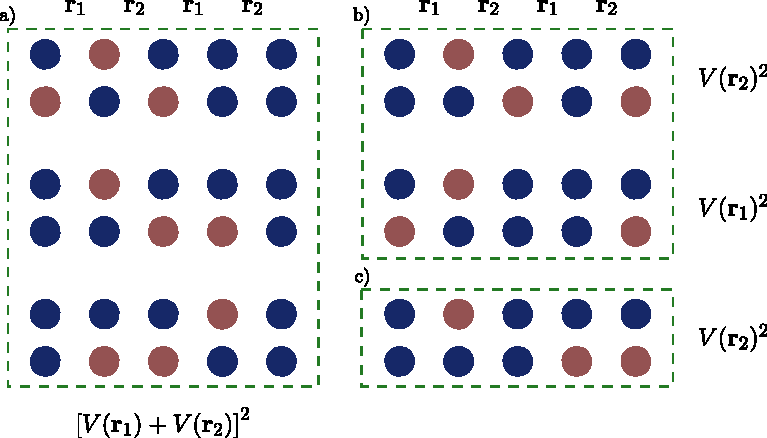
\includegraphics{pictures/SWT_calc.pdf}
    \caption{\textbf{Coupling schemes.} There are different ways double excited states couple to the single excited ones. The top row always depicts a state of the single, while the bottom row depicts a state of the double excited subspace. Generally configurations of two different subspaces are coupled to each other, when for two neighboring atoms one configuration has the inverted excitation scheme with respect to the other. I assign them to three categories. The first category is depicted in a). It couples two neighboring atoms twice. In the picture all possible cases are shown. For b) only two atoms couple two each other. Here the coupling takes place at a pair of $\ket{e}$ and $\ket{g}$ in both configurations. If the excitation in the single excitation subspace is at position $2<i<N-1$, there are $N-4$ different states in the double excited subspace that contribute a term $V(\mathbf{r}_1)^2$ and the same number for $V(\mathbf{r}_2)^2$. Category c) couples two unexcited sites in the single excitations subspace to two excited sites in the double excited subspace. For this case there are $N/2-2$ states that contribute $V(\mathbf{r}_1)^2$ and  $N/2-2$ states that contribute $V(\mathbf{r}_2)^2$, if the single excited state is is excited at atom $2<i<N-1$.}
    \label{fig:SWT_schemes}
\end{figure}
In the following the effective Hamiltonian will be calculated for the specific configuration we are looking at. We consider a one-dimensional staggered chain of $N$ atoms, where the atoms are separated by alternating distances $\mathbf{r}_1$ and $\mathbf{r}_2$. For a single atom there are only two states available, excited $\ket{e}$ and unexcited $\ket{g}$. The states $\ket{i}$, which are summed over, represent the states where only atom $i$ is excited and the others are in the unexcited state. Going to a regime where only nearest neighbor interactions contribute we can write using the coupling schemes of \figref{fig:SWT_schemes}
\begin{align*}
    H_{\text{eff},2}&= \sum_{i=1}^N\tilde{V}_i\,\ket{i}\bra{i}\\
    \tilde{V}_i &=-\frac{1}{\Delta}\,\begin{cases}
        3\,\left[V(\mathbf{r}_1)+V(\mathbf{r}_2)\right]^2+(N-4+\frac{N}{2}-2)\,V^2(\mathbf{r}_1)+(N-4+\frac{N}{2}-2)\,V^2(\mathbf{r}_2)&\text{if}\;1\neq i\neq N\\\\
        \left[V(\mathbf{r}_1)+V(\mathbf{r}_2)\right]^2+(N-3+\frac{N}{2}-1)\,V^2(\mathbf{r}_1)+(\frac{N}{2}-1)\,V^2(\mathbf{r}_2)&\text{if}\;i=1\\\\
        2\,\left[V(\mathbf{r}_1)+V(\mathbf{r}_2)\right]^2+(N-3+\frac{N}{2}-2)\,V^2(\mathbf{r}_1)+(N-4+\frac{N}{2}-1)\,V^2(\mathbf{r}_2)&\text{if}\;i=2\\\\
        2\,\left[V(\mathbf{r}_1)+V(\mathbf{r}_2)\right]^2+(N-4+\frac{N}{2}-1)\,V^2(\mathbf{r}_1)+(N-3+\frac{N}{2}-2)\,V^2(\mathbf{r}_2)&\text{if}\;i=N-1\\\\
        \left[V(\mathbf{r}_1)+V(\mathbf{r}_2)\right]^2+(\frac{N}{2}-1)\,V^2(\mathbf{r}_1)+(N-3+\frac{N}{2}-1)\,V^2(\mathbf{r}_2)&\text{if}\;i=N
    \end{cases}
\end{align*}
% There is actually another case distinction necessary for $i=2$ and $i=N-1$, this will be clearer later.
The part involving interactions within the same subspace can be written as 
\begin{align*}
    P_0VP_0&= \sum_{\substack{i=1\\j=i+1}}^{N-1} V(\mathbf{r}_{i,j})\,\sigma^+_i\sigma^-_j+\text{h.c.},
\end{align*}
where $\mathbf{r}_{i,j}$ is the distance between the $i$th and $j$th site. I now also want to write $H_{\text{eff},2}$ in terms of a sum of two atom operators. Therefore I introduce the projectors $n^e_i=\ket{e}_i\bra{e}_i$ and $n^g_i=\ket{g}_i\bra{g}_i$.
\begin{align*}
    H_{\text{eff},2}&=\sum_{\substack{i=1\\j=i+1}}^{N-1}V^2(\mathbf{r}_{i,j})\,(n^e_in^g_j + n^g_in^e_j + n^g_in^g_j)+\sum_{i=2}^{N-1}\left[ V(\mathbf{r}_{i-1,i})+V(\mathbf{r}_{i,i+1}) \right]^2 \, n^g_{i-1}n^e_in^g_{i+1}\\ &+\sum_{i=3}^{N-1} \left[ V(\mathbf{r}_{i-2,i-1})+V(\mathbf{r}_{i-1,i}) \right]^2 \, n^g_{i-2}n^g_{i-1}n^e_{i} 
    +\sum_{i=2}^{N-2} \left[ V(\mathbf{r}_{i,i+1})+V(\mathbf{r}_{i+1,i+2}) \right]^2 \, n^e_{i}n^g_{i+1}n^g_{i+2} \\
    &+ \left[ V(\mathbf{r}_{1,2})+V(\mathbf{r}_{2,3}) \right]^2 n^e_1n^g_2n^g_3 + \left[ V(\mathbf{r}_{N-2,N-1})+V(\mathbf{r}_{N-1,N}) \right]^2 n^g_{N-2}n^g_{N-1}n^e_{N}
\end{align*}
A last step is possible since in the single excitation subspace terms like $n^e_in^g_j$ simplify to just $n^e_i$.
\begin{align*}
    &= \sum_{i=2}^{N-1}\left(V^2(\mathbf{r}_{i-1,i})+V^2(\mathbf{r}_{i,i+1})+\left[ V(\mathbf{r}_{i-1,i})+V(\mathbf{r}_{i,i+1}) \right]^2 \right)\,n^e_i \\&+ \sum_{i=3}^{N-1} \left[ V(\mathbf{r}_{i-2,i-1})+V(\mathbf{r}_{i-1,i}) \right]^2\, n^e_i +\sum_{i=2}^{N-2} \left[ V(\mathbf{r}_{i,i+1})+V(\mathbf{r}_{i+1,i+2}) \right]^2\,n^e_i\\
    &+ \left( V^2(\mathbf{r}_{1,2}) + \left[ V(\mathbf{r}_{1,2})+V(\mathbf{r}_{2,3}) \right]^2 \right)\,n^e_1 + \left( V^2(\mathbf{r}_{N-1,N})+ \left[ V(\mathbf{r}_{N-2,N-1})+V(\mathbf{r}_{N-1,N}) \right]^2\right)\,n^e_N\\
    &+ \sum_{i=1}^{N-1} V(\mathbf{r}_{i,i+1})\,n^g_in^g_{i+1}
\end{align*}
\subsection*{Energy scales}
The most important energies which determine the dynamics are the trap frequency, which is of the order $\omega\sim10\,\text{-}\,100\,\text{kHz}$, the distances between atoms who can reliably reach $3\,\mu\text{m}$, and the lifetime of the Rydberg states, which is in the order of $100\,\mu\text{s}$. From this it already becomes apparent that, in order to see dynamics of the system within the lifetime of the Rydberg states, the coupling strength has to be higher than the trap frequency. This prevents the Lamb-Dicke regime, as the phonon number cannot be assumed as conserved. Thus the first order expansion in the deplacements of the atoms has to be taken into account. The relative size of each order of the expansion can be estimated by the factor
\begin{align*}
    \varepsilon\vcentcolon=\sqrt{\frac{\hbar}{m\omega}}\,\frac1r\approx(2\,\text{-}\,11)\cdot10^{-3}
\end{align*}
As the dipole interaction is a function of the angle $\vartheta$ between the dipole moment and the axis of the chain, the interaction can be tuned in a way that the first order term vanishes. As can be seen in \figref{fig:dipole_orientation_for_vanishing_first_order}, the second order term in the expansion is of the order $5\cdot10^{-5}\,\text{-}\,10^{-3}$, smaller than the leading order. 
\begin{figure}[H]
    \centering
    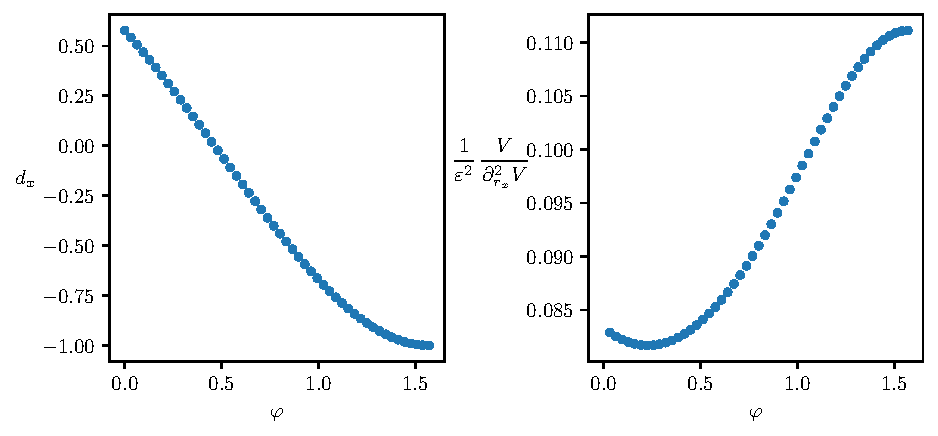
\includegraphics{pictures/magnitude_dersqV_ifderVzero.pdf}
    \caption{\textbf{Dipole orientation and ratio of interactions.} For all angles $\sin\varphi\vcentcolon=h/r$ one can find a dipole orientation, shown in the left panel, such thatthe first order term in the expansion of the interaction vanishes. The ratio between zeroth order and second order term is shown in the right panel. }
    \label{fig:dipole_orientation_for_vanishing_first_order}
\end{figure}




\subsection*{First order approximation in spin degrees}
For the first approach I will continue with the Hamiltonian up to first order in the dipole interaction, i.e. without $H_{\text{eff},2}$. The phonons are introduced by again expanding the interaction up to second order. When we choose the dipole orientation, such that thr first order vanishes, the Hamiltonian reads
\begin{align*}
    H&= \sum_{i=1}^{N-1}\left[V(\mathbf{r}_{i,i+1})+\frac12\,\sum_{n,m\in\{i,i+1\}}\frac{\partial^2V(\mathbf{r}_{i,i+1})}{\partial\mathbf{r}_{n}\partial\mathbf{r}_m}\,\delta\mathbf{\hat{r}}_n\delta\mathbf{\hat{r}}_m\right]\,\sigma_i^+\sigma_{i+1}^-+\text{h.c.}\\
    &= \sum_{i=1}^{N-1}\left[V(\mathbf{r}_{i,i+1})-\frac{\hbar}{2m\omega}\,\frac{\partial^2V(\mathbf{r}_{i,i+1})}{\partial\mathbf{r}_{i}^2}\,\left(p_j^\dagger p_{j+1}+p_{j+1}^\dagger p_{j}-p_{j}^\dagger p_{j}-p_{j+1}^\dagger p_{j+1}\right)\right]\,\sigma_i^+\sigma_{i+1}^-+\text{h.c.}
\end{align*}
The quadrature operators of the phonons are used $\delta\mathbf{\hat{r}}_i=\sqrt{\frac{\hbar}{2m\omega}}\,(p_i + p_i^\dagger)$. In the following I want to present a brief investigation of the influence of this small second order term on the dynamics of the spins. Ultimately I am interested in the effect of the phonons on the transport of spin excitations via a Rice-Mele scheme. Therefore I will compare the free evolution of the system with and without phonons at conditions mimicking a point in the middle of the Rice-Mele cycle, where the dynamics are the fastest. The results are shown in \figref{fig:diff_free_evol_with_without_phonons}. As can be seen, for high phonon excitation numbers the difference in the spin excitations during the time period of the whole cycle becomes substantial. Nevertheless, the performance of the Rice-Mele protocol is affected only mildly, and is even slightly improved by the inclusion of the phonons, as can be seen in \figref{fig:end_excitation_rice_mele_with_without_phonons}.

\begin{figure}[H]
    \hspace*{-1.5cm}
    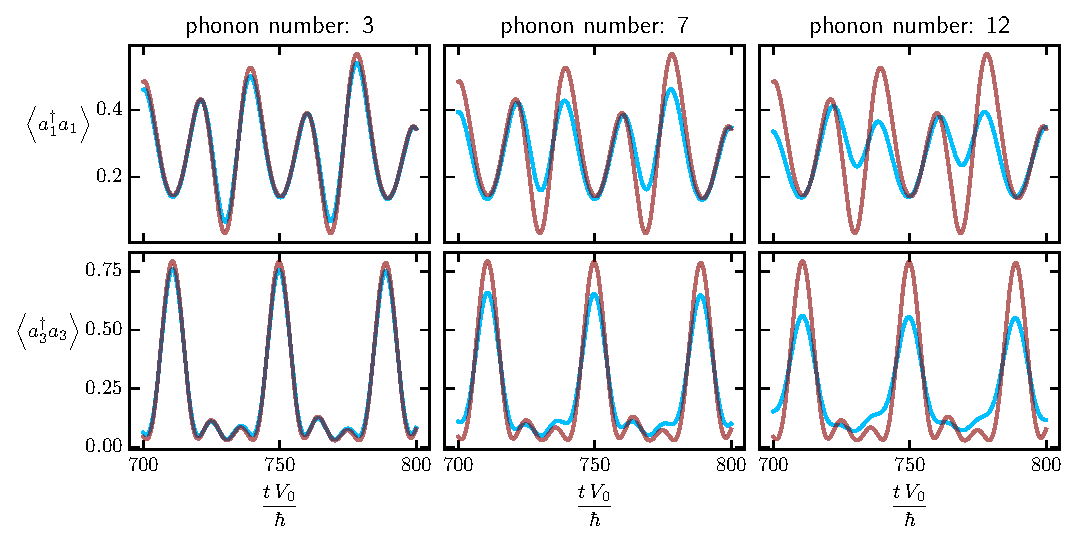
\includegraphics{pictures/compare_with_without_phonon_late_time.pdf}
    \caption{\textbf{Comparison of free evolution with and without phonons.} The difference in spin excitation probability between the free evolution with and without phonons is shown for a chain of length $N=4$. As initial conditions I chose a quadratically decaying excitation profile from the right edge and parameters $b=1.2\,r_0$, $h=0.4\,r_0$, $a=3\,r_0$. The red line shows the trajectory for the case without motional degrees of freedom and the blue one the case with phonons present.For an atom with 12 motional excitations the mean displacement is of the order of $0.15\,\mu\text{m}$, which is already around the limit of the expansion to second order being accurate.}
    \label{fig:diff_free_evol_with_without_phonons}
\end{figure}

\begin{figure}[H]
    \hspace*{-1.5cm}
    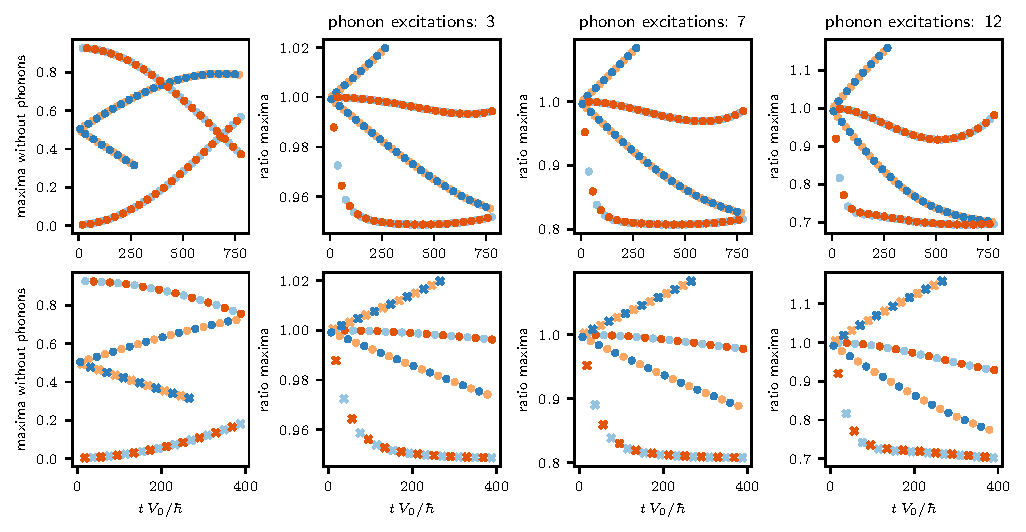
\includegraphics{pictures/maxima_compared_free_evolution.pdf}
    \caption{\textbf{Comparison of the maxima of the free evolution with and without phonons.} For the same parameters and initial conditions as in \figref{fig:diff_free_evol_with_without_phonons} the maxima of the spin excitation probability at the individual sites are compared for the free evolution with and without phonons. }
    % \label{fig:diff_free_evol_with_without_phonons}
\end{figure}

\begin{figure}[H]
    \centering
    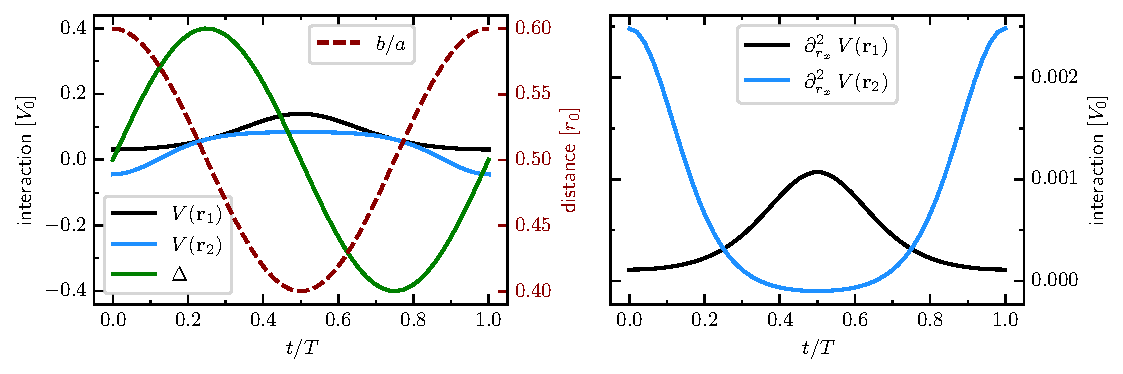
\includegraphics{pictures/rice-mele-scheme1to1000.pdf}
    \caption{\textbf{Rice-Mele scheme.} Depicted is the course of the the decisive parameters during the Rice-Mele cycle, i.e. the axial distance between atoms in the unit cell $b=1.8\,\text{-}\,1.2\,\text{-}\,1.8\,r_0$ (the distance orthogonal to the chain axis is kept constant $h=0.4\,r_0$ as well as the distance inside a sublattice $a=3\,r_0$). The detuning takes it's maximal value at $\Delta_\text{max}=0.4\,V_0$.}
    % \label{fig:end_excitation_rice_mele_with_without_phonons}
\end{figure}

\begin{figure}[H]
    \centering
    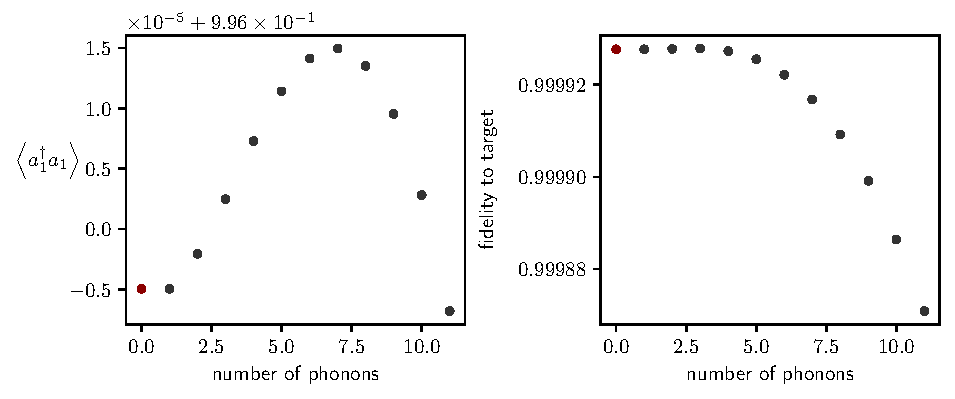
\includegraphics{pictures/transfered_excitation_depphon.pdf}
    \caption{\textbf{Transfered excitation in dependence of phonon number.} I show the excitation probability at the left edge at the end of the cycle, when the system is initialized in an eigenstate of the pure spin Hamiltonian localized at the right edge. And parameters of the cycle are $b=1.8\,\text{-}\,1.2\,\text{-}\,1.8\,r_0$, $h=0.4\,r_0$, $a=3\,r_0$, $\Delta_\text{max}=0.4\,V_0$.}
    \label{fig:end_excitation_rice_mele_with_without_phonons}
\end{figure}